\documentclass[journal]{IEEEtran}
\usepackage{epsf,cite,amsmath,amscd,graphics,graphicx,latexsym,multicol,setspace}
\usepackage{amsfonts,amsmath,amssymb,amsthm}
\usepackage{scalefnt}
\newcounter{MYtempeqncnt}
\begin{document}
\title{Twitter Sentiment Analysis with Recurrent Neural
Networks}

\author{Mahtab Tamannaee, Kandasamy Illanko\\
\{Mahtab, killanko\}@ryerson.ca\\
Department of Electrical and Computer Engineering\\
Ryerson University, Toronto, Canada.}
\maketitle
\begin{abstract}
One of the most popular topic in the field of deep learning and natural language processing is Sentiment analysis. Sentiment classification in natural language texts is a classification task of finding the polarity of the sentiments before them. One of the best sources of Natural Language texts and the most challenging one is the twitter database. Similar to the other NLP tasks, the deep learning methods have outperformed the other well-known NLP tasks.
In this project, we address the document-level sentiment classification task and explore the application of Recurrent Neural Networks on this task from both deep learning and natural language processing point of view. Finally we provide a model by a special type of RNN, Long Short Term Memory network RNN architecture to perform predictions and analysis. This conducted evaluations show that our model is efficient and making it practical classification. Our model reached 77 percent accuracy on 1,600,000 tweets data-set.

\end{abstract}
\begin{IEEEkeywords}
Sentiment Analysis, Recurrent Neural Networks, Artificial Intelligence
\end{IEEEkeywords}

\section{Introduction}
\label{intro}

This ability to identify the positive or negative sentiment behind a text is interesting when it comes to social media like twitter. A predictive model could predict sentiment polarities of live tweets which would identifies the user's attitude  towards an event. Performing classification with social media data can be challenging as most of the natural language texts in social media include hyperlinks, mentions, or other non-text contents. The contents of each will help the user to include more concept into a tweet or review. However, such content are not structured enough for the machine to learn. The employment of pre-processing ease up the procedure of converting these contents into structured data\cite{Mabrouk}. Similar to any Machine Learning model, its important to choose and use proper features to train models. Some studies have proved that working on the feature selection stage can potentially improve the classification accuracy. Word embedding and language models are typically applied for feature representation in deep Learning approaches.\cite{Mabrouk}

A Neural Network Model inputs the words into the input nodes (like word embedding) and the output values of nodes predicts the classification results. Basically, there are two original types of NN architectures that try to capture semantic and syntactic information as follows:
\begin{itemize}
  \item Convolutional Neural Networks (CNN) is a Feed-Forward Neural Network which has the advantage of being able to handle high computational cost of NN. However, it needs more training time in comparison to backward Neural Network.
  \item Recurrent Neural Networks (RNN) is a Backward Neural Network. In this network the output of one state is dependant of its previous state. This model requires large space to train properly. This dependency makes the RNN more superior in learning sequential information. Another advantage of RNN is that reduces the number of parameters as it keeps the same parameters at each step. 
  
\end{itemize}

\bigskip
As we concluded, unlike feed forward neural networks, RNN can use its internal “memory” to learn a sequence of inputs,	which	 makes it popular for processing sequential data.\cite{ZhangL}. Recurrent models match people’s intuition of reading word by word and are capable to model the intrinsic relations between sentences. Without any explicit boundary, RNNs could extract the sentence representation and analyze the semantic meaning of it at the same time keeping the word sequence.\cite{XuJ} The advantages of RNN over CNN encouraged us to choose this it for modeling our sentiment classifier. 
In the next section, we provide a literature review about most important paper works in this domain. The problem statement and our proposed models will be discussed in section \ref{sysmo}. In section \ref{experi} we will demonstrate the experiments performed and will analyse the evaluation results.


\section{Related Work}
\label{related}
RNN models have been widely used in Sentiment Classification. There have been several attempts to solve classification problem using machine learning. In this section, we briefly review and discuss the major researches conducted that are relevant to this work. The LSTM models have been shown the best performance between other CNN based methods\cite{Mabrouk}. Some of the best designs and state of arts are given here and they are all based on LSTM models.
\mdskip

Authors in \cite{XuJ}, proposed a model named as Cached LSTM which improves the LSTM ability to carry information for long distances. they presented Cached Long Short-Term Memory neural networks (CLSTM) to capture the overall semantic information in long texts. CLSTM provides a cache mechanism, which divides memory into several groups with different forgetting rates and thus enables the network to keep the document's sentiment information better within a recurrent unit. 
\mdskip

The authors in \cite{Tang} , proposed a model named as NCSL which includes two target dependent long short-term memory (LSTM) models. Neural Context-Sensitive Lexicon utilizes sentiment lexicons to treat the sentiment score of a sentence as a weighted sum of prior sentiment scores of negation words and sentiment words.  
\mdskip

In this article \cite{Wang} ,the authors proposed an attention-based model named as TD-LSTM for aspect-level sentiment classification task. They approach this task by an idea of learning aspect embeddings and let aspects participate in computing attention weights
Target-dependent LSTM treats an aspect as a target by using two LSTM surrounding the aspect term. Such model allows different aspects to be given as it concentrate on different parts of a sentence for different aspects.
\mdskip

Ruder S et.al in \cite{Ruder} proposed a hierarchical model named as TC-LSTM. This model performs aspect-based sentiment analysis by modeling the interdependencies of sentences in a review with a hierarchical bidirectional LSTM.  Target-connection LSTM  facilitates TD-LSTM to learn the relationship between aspect and each context word. They demonstrate this hypothesis for the task of aspect-based sentiment analysis by modeling the interdependencies of sentences in a review with a hierarchical bidirectional LSTM.
\mdskip

Yi Tay et. al in \cite{Tay} , proposed a model named as ATAE-LSTM. Attention-based LSTM with Aspect Embedding consists of aspect attention vector with LSTM hidden vector for the sentiment polarity. By looking at word-aspect associative relationships, they incorporate aspect information into the neural model.In order to model the similarity between aspect and words, they employed a circular convolution and circular correlation. 
\mdskip

Yang Z et.al in \cite{Yang}, proposed a model named as Aspect-fusion LSTM. This AF-LSTM model is hierarchical attention networks (HAN) for classifying document.  They used an additional attention mechanism and learns associative relationships between aspect and context words by word-aspect fusion attention. The document vector gets constructed in a hierarchical order first by aggregating important words into sentence vectors, and then aggregating important sentences vectors to document vectors. 

\section{Dataset}
We choose sentiment140 (Fig \ref{fig:dataset}), as the base dataset for model development and intuition. Most of the baselines methods are used a social media datasets, we also used twitter dataset for comparison purposes. This dataset consists of 1,600,000 tweets.

\begin{figure}[t]
\centering
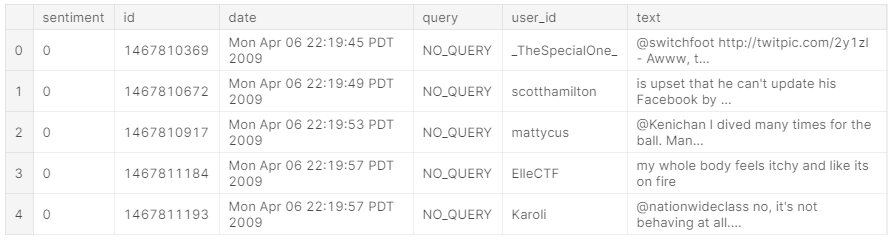
\includegraphics[width=1\columnwidth]{Dataset.PNG}
\caption{\small Twitter Sentiment140 data-set schema.}
    \label{fig:dataset}
\end{figure}


Different scores,from the range of zero to four, have been assigned to these tweets . Based on such score assignment, score = 0 indicates the most negative polarity score, and the score = 4 indicates the most positive polarity score. As you can see in Fig \ref{fig:datasetstat}, by mapping the Negative polarity to tweets that their score is zero and positive polarity to the ones with score of 4, we can construct our data set with 800,000 positive tweets and 800,000 negative tweets. 


\begin{figure}[t]
\centering
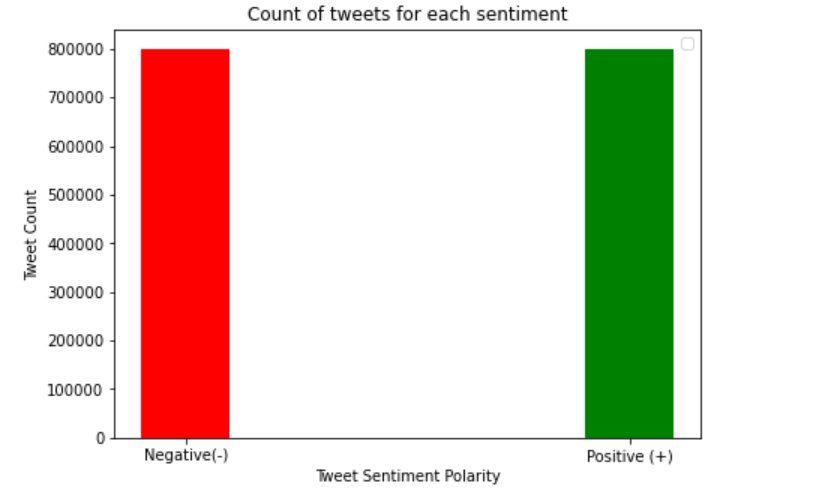
\includegraphics[width=1\columnwidth]{Dataset Lable Dist.PNG}
\caption{\small Twitter Sentiment140 positive and negative polarities.}
    \label{fig:datasetstat}
\end{figure}

We further divided the data set into a train set of size 1280000 and a test set of size 320000.


\section{System Model and the Problem Statement}
\label{sysmo}
Sentiment Analysis has been studied at three levels, document level, sentence level, and aspect level\cite{Yang}. In this project we perform Document level sentiment classification which classifies the sentiment behind a document(ex. tweet, query, or text) to a polarity, negative or positive. This type of sentiment classification can be considered under document classification category in NLP. This opinion classification is a conclusion on overall sentiment of the document. Such sentiment analysis can also understood as a regression task if the model needs to predict a rating score of a review or tweet.

\subsection{ Dense Document Vector Representation : Word2Vec}
To perform sentiment analysis on document level, we need to express each document with a dense representation which can convey contextual information of each document term with respect to the text its extracted from. For such purpose, language modeling have shown promising word contextual modeling which provide word embedding representations. Employing the word embedding representations constructs a dense document vector which can be used as perfect feature of a document.

\mdskip
For such purpose, a local word embedding model (Word2Vec) was trained and used to construct the embedding layer representing the feature of each text or tweet. The Word2Vec word embedding model has been built using the well known GENSIM Python library.

\subsection{ Long Short-Term Memory RNN : LSTM}
We propose a architecture for twitter sentiment classification at document-level by utilizing a special type of recurrent neural networks (RNN),  Long Short Term Memory network. The main idea is to use such networks to learn sequential pattern and context of tweets and predict a numerical value which further can be mapped into polarity classification.. This network can handle the processing of long-term dependencies. This advantage comes from  the repeating module of LSTM structure which employs four layers of neural network. The LSTM model provides two cell states and decides the output based on cell states. This model uses sigmoid layer. \cite{Yang}.

\bigskip

In Long short-term memory network (LSTM),  Considering  $\mathcal{ \sigma}$ as is the logistic sigmoid function, and$\mathcal{ \odot}$ is the element-wise multiplication operation, the update of each LSTM Model component can be formalized as:

\bigskip

\begin{array}{l}
\mathbf{i}^{(t)}=\sigma\left(\mathbf{W}_{i} \mathbf{x}^{(t)}+\mathbf{U}_{i} \mathbf{h}^{(t-1)}\right) \\
\mathbf{f}^{(t)}=\sigma\left(\mathbf{W}_{f} \mathbf{x}^{(t)}+\mathbf{U}_{f} \mathbf{h}^{(t-1)}\right) \\
\mathbf{o}^{(t)}=\sigma\left(\mathbf{W}_{o} \mathbf{x}^{(t)}+\mathbf{U}_{o} \mathbf{h}^{(t-1)}\right) \\
\tilde{\mathbf{c}}^{(t)}=\tanh \left(\mathbf{W}_{c} \mathbf{x}^{(t)}+\mathbf{U}_{c} \mathbf{h}^{(t-1)}\right) \\
\mathbf{c}^{(t)}=\mathbf{f}^{(t)} \odot \mathbf{c}^{(t-1)}+\mathbf{i}^{(t)} \odot \tilde{\mathbf{c}}^{(t)} \\
\mathbf{h}^{(t)}=\mathbf{o}^{(t)} \odot \tanh \left(\mathbf{c}^{(t)}\right)
\end{array}

\bigskip

 Considering the gates,  $\mathbf{i}^{(t)}, \mathbf{f}^{(t)}, \mathbf{o}^{(t)}$ and $\mathbf{c}^{(t)}$ as the input gate, forget gate, output gate, and memory cell activation vector at time-step $t$ respectively.
 letting $H$ as dimensionality of hidden layer and $d$ as dimensionality of input, $\mathbf{h}^{(t)}$ corresponds to hidden vector.$\mathbf{h}^{(t)} \in \mathbb{R}^{H} . \mathbf{W}_{i}, \mathbf{W}_{f}$. $\mathbf{W}_{o} \in \mathbb{R}^{H \times d}$ and $\mathbf{U}_{i}, \mathbf{U}_{f}, \mathbf{U}_{o} \in \mathbb{R}^{H \times H}$ are train-able parameters. 


\section{Experiments}
the RNN should have the following architecture which includes EmbeddingLayer, LSTM, and Dense layer. Since we are going to build a sequence model. We should feed in a sequence of numbers to it.These sequence of numbers are the sequence of word embedding of the terms in each tweet.

\mdskip

This NN classifier outputs a scalar value prediction. This model predicts an score between 0 and 1. Specifying a THRESHOLD will provide classification of the sentiment being positive if the predicted value is above THRESHOLD. In this project, the THRESHOLD has been set to "0.5", therefore, a tweet gets classified as POSITIVE if its predicted value is above "0.5".

\mdskip

Two callbacks gets called at the end of each epoch: First, ReduceLROnPlateau, which updates a Learning Rate at specific epoch. Second, EarlyStopping, which allows a performance measure to be specified and monitored. And steppes the training if it gets triggered.

\begin{figure}[t]
\centering
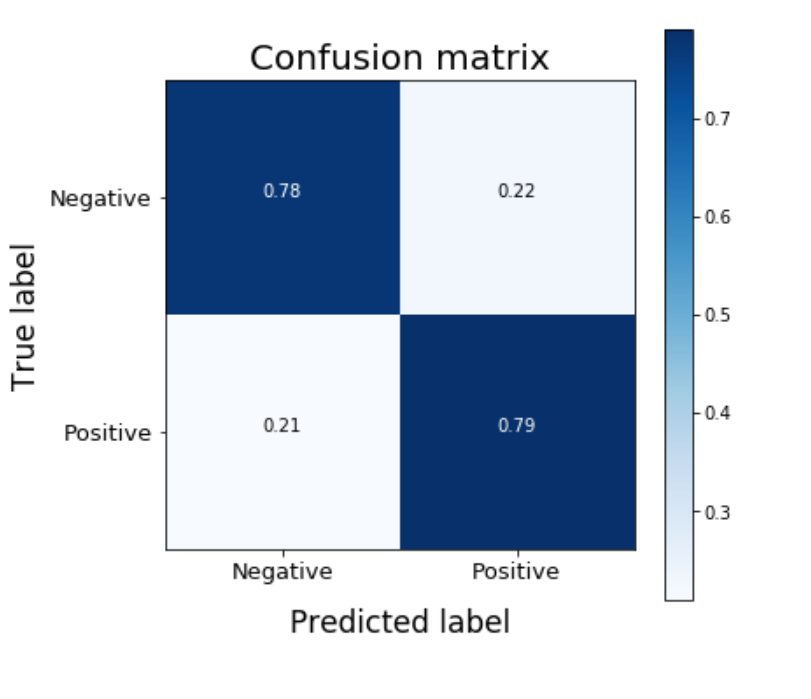
\includegraphics[width=1\columnwidth]{CMat.png}
\caption{\small Confusion Matrix of model classification.}
    \label{fig:cmat}
\end{figure}


\begin{figure}[t]
\centering
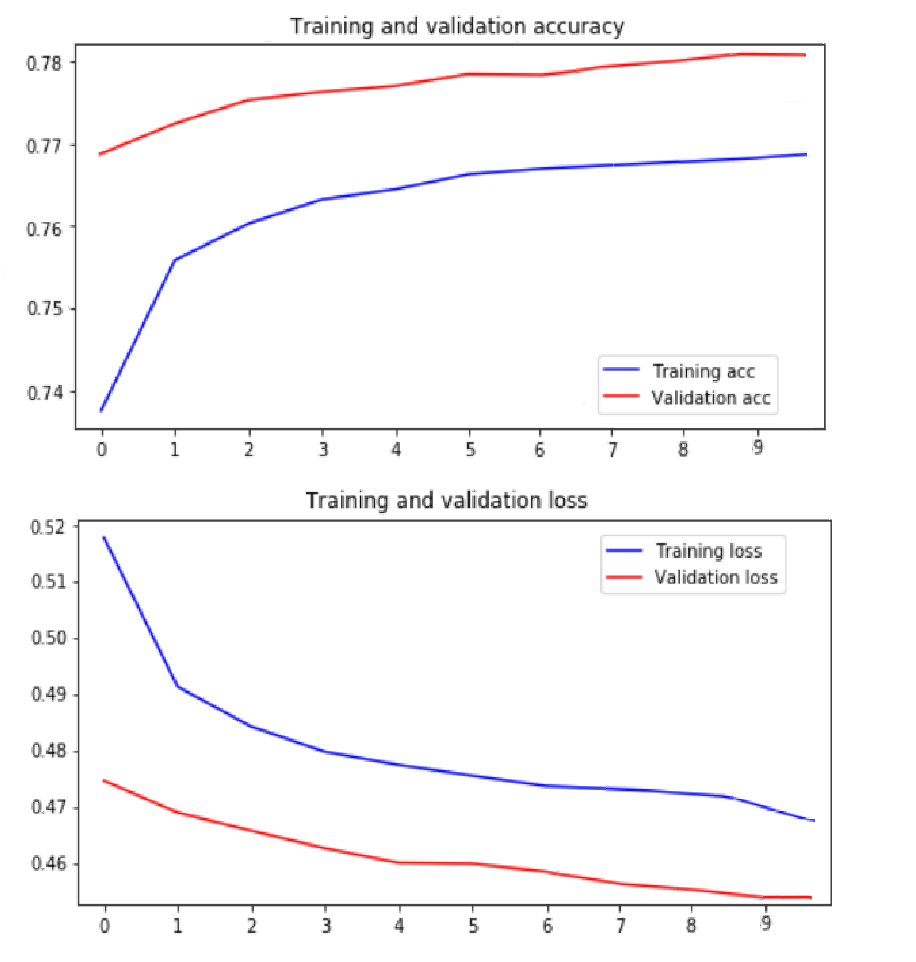
\includegraphics[width=1\columnwidth]{Accuracy Loss.png}
\caption{\small Twitter Sentiment140 positive and negative polarities.}
    \label{fig:accuracyloss}
\end{figure}



\subsection{Accuracy and Loss Results and Analysis} accuracyloss
In the first step of evaluation, Learning Curve of loss and accuracy of the model on each epoch has been graphed. According to the Fig  \ref{fig:accuracyloss} we can see the accuracy and loss of the model on each epoch. Its crystal clear that the accuracy of the validation set has reached  has reach 77 percent. Similarly the value of the loss has declined to 0.4601. Similar trend on both training and validation dataset shows promising facts that the model is not over-fitted or remained untrained.


\subsection{Classification Results and Analysis}
The classification accuracy, Precision, Recall, and f1-score has been reported in Table 1. The values of the table is compatible with the Confusion Matrix (Fig Fig  \ref{fig:cmat}) which shows the true positive, false positive, true negative, and false negative classifications. 


\begin{table}[]
\caption{Classification Result summery}
\label{tab:my-table}
\begin{tabular}{|l|l|l|l|l|}
\hline
- & precision & recall & f1-score & support \\ \hline
Negative & 0.78 & 0.76 & 0.77 & 160539 \\ \hline
Positive & 0.77 & 0.77 & 0.77 & 159461 \\ \hline
Accuracy & - & - & 0.77 & 320000 \\ \hline
macro avg & 0.77 & 0.77 & 0.77 & 320000 \\ \hline
weighted avg & 0.77 & 0.77 & 0.77 & 320000 \\ \hline
\end{tabular}
\end{table}





\section{Conclusion}
In this paper, we applied a LSTM RNN on twitter data to observe the accuracy of this architecture to perform  document-level sentiment classification. Building a language model based on local data set data has been shown effective as it provided dense document representation of documents. Training and testing the LSTM model on dense document embedding has reached 77 percent accuracy on 1,600,000 tweeter database.  


\begin{thebibliography}{20}


\bibitem{Mabrouk}
A. Mabrouk, R. P. D. Redondo and M. Kayed, "Deep Learning-Based Sentiment Classification: A Comparative Survey," in IEEE Access, vol. 8, pp. 85616-85638, 2020, doi: 10.1109/ACCESS.2020.2992013.

\bibitem{Deng}
Z.-H. Deng, K.-H. Luo and H.-L. Yu, "A study of supervised term weighting scheme for sentiment analysis", Expert Syst. Appl., vol. 41, no. 7, pp. 3506-3513, Jun. 2014.


\bibitem{XuJ}
Xu J, Chen D, Qiu X, Huang X. Cached long short-term memory neural networks for document-level sentiment classification. arXiv preprint arXiv:1610.04989. 2016 Oct 17


\bibitem{Tang}
Tang D, Qin B, Feng X, Liu T. Effective LSTMs for target-dependent sentiment classification. arXiv preprint arXiv:1512.01100. 2015 Dec 3.


\bibitem{Wang}
Wang Y, Huang M, Zhu X, Zhao L. Attention-based LSTM for aspect-level sentiment classification. InProceedings of the 2016 conference on empirical methods in natural language processing 2016 Nov (pp. 606-615).


\bibitem{Ruder}
Ruder S, Ghaffari P, Breslin JG. A hierarchical model of reviews for aspect-based sentiment analysis. arXiv preprint arXiv:1609.02745. 2016 Sep 9.


\bibitem{Tay}
Tay Y, Tuan LA, Hui SC. Learning to attend via word-aspect associative fusion for aspect-based sentiment analysis. InThirty-second AAAI conference on artificial intelligence 2018 Apr 26.


\bibitem{Yang}
Yang Z, Yang D, Dyer C, He X, Smola A, Hovy E. Hierarchical attention networks for document classification. In Proceedings of the 2016 conference of the North American chapter of the association for computational linguistics: human language technologies 2016 Jun (pp. 1480-1489).


\bibitem{ZhangL}
Zhang L, Wang S, Liu B. Deep learning for sentiment analysis: A survey. Wiley Interdisciplinary Reviews: Data Mining and Knowledge Discovery. 2018 Jul;8(4):e1253.






\end{thebibliography}
\end{document}

